%%% LaTeX Template
%%% This template can be used for both articles and reports.
%%%
%%% Copyright: http://www.howtotex.com/
%%% Date: February 2011

%%% Preamble
\documentclass[paper=a4, fontsize=11pt]{scrartcl}	% Article class of KOMA-script with 11pt font and a4 format

\usepackage[english]{babel}															% English language/hyphenation
\usepackage[protrusion=true,expansion=true]{microtype}				% Better typography
\usepackage{amsmath,amsfonts,amsthm}										% Math packages
\usepackage[pdftex]{graphicx}														% Enable pdflatex
%\usepackage{color,transparent}													% If you use color and/or transparency
\usepackage[hang, small,labelfont=bf,up,textfont=it,up]{caption}	% Custom captions under/above floats
\usepackage{epstopdf}																	% Converts .eps to .pdf
\usepackage{subfig}																		% Subfigures
\usepackage{booktabs}																	% Nicer tables


%%% Advanced verbatim environment
\usepackage{verbatim}
\usepackage{fancyvrb}
\DefineShortVerb{\|}								% delimiter to display inline verbatim text


%%% Custom sectioning (sectsty package)
\usepackage{sectsty}								% Custom sectioning (see below)
\allsectionsfont{%									% Change font of al section commands
	\usefont{OT1}{bch}{b}{n}%					% bch-b-n: CharterBT-Bold font
%	\hspace{15pt}%									% Uncomment for indentation
	}

\sectionfont{%										% Change font of \section command
	\usefont{OT1}{bch}{b}{n}%					% bch-b-n: CharterBT-Bold font
	\sectionrule{0pt}{0pt}{-5pt}{0.8pt}%	% Horizontal rule below section
	}


%%% Custom headers/footers (fancyhdr package)
\usepackage{fancyhdr}
\pagestyle{fancyplain}
\fancyhead{}														% No page header
\fancyfoot[C]{\thepage}										% Pagenumbering at center of footer
\renewcommand{\headrulewidth}{0pt}				% Remove header underlines
\renewcommand{\footrulewidth}{0pt}				% Remove footer underlines
\setlength{\headheight}{13.6pt}

%%% Equation and float numbering
\numberwithin{equation}{section}															% Equationnumbering: section.eq#
\numberwithin{figure}{section}																% Figurenumbering: section.fig#
\numberwithin{table}{section}																% Tablenumbering: section.tab#
\usepackage[parfill]{parskip}
\usepackage{float}
\usepackage{graphicx}

%%% Title	
\title{ \vspace{-1in} 	\usefont{OT1}{bch}{b}{n}
		\huge \strut An overview of indirect inelastic data analysis within Mantid\strut \\
}
\author{ 									\usefont{OT1}{bch}{m}{n}
        Samuel Jackson\\		\usefont{OT1}{bch}{m}{n}
		ISIS Facility\\	\usefont{OT1}{bch}{m}{n}
        STFC Rutherford Appleton Laboratory\\
        \texttt{samuel.jackson@stfc.ac.uk}
}
\date{\today}

%%% Begin document
\begin{document}
\maketitle
\clearpage
\tableofcontents
\section{Introduction}
Mantid (http://www.mantidproject.org/) is an open source, cross platform framework for the analysis of Neutron and Muon scattering data. The project is primarily written in C++ with a Python API. The project includes a GUI based off of the QtiPlot project and primarily written using the Qt library.

Mantid aims to provide a single platform for neutron and muon scattering data analysis to all facilities across the world. It is developed by two teams of developers, one based at the ISIS facility at Rutherford Appleton Laboratory UK, the other at the SNS facility at Oakridge USA. Recently additional partners from the ILL and PSI have also contributed.

The project is currently still under heavy development and provides regular incremental releases for evaluation and feedback from instrument scientists and users in general and is therefore constantly evolving with each release. Until recently, Mantid operated on a three month release cycle. This has now been changed to so that the project releases every four months, with a longer emphasis on the testing and integration phase of development.

Up until now the indirect inelastic section of Mantid has largely been based off of the the existing MODES application which in turn was based on OpenGenie\cite{wshowells2010}. The majority of the functionality has now been integrated into the Mantid framework in form or another and we are now beginning to reach a point where we can expand the functionality offered further.

This document aims to give an overview of the current stage of development for the indirect inelastic section of the application as it currently exists, beginning with an introduction the relevant background material and progressing to the outline the existing system. We then provide a weak outline of suggested directions for further development in the near future.

\section{A Brief Introduction to Neutron Scattering}
Neutron scattering experiments are used to probe the structure of materials at a fundamental level. The results of such experiments can be used to learn a great deal about the internal structure of a sample and how it can behave under different conditions. In a neutron scattering experiment, a beam of neutrons is produced at a source (such as the one provided by ISIS) and directed to the various instruments attached to the beam line. These neutrons then scatter from the sample placed in the instrument. The angle and energy at which scattered neutrons are detected can then be used to deduce the structure and dynamics of the sample.

There are two main types of neutron scattering: elastic and inelastic. Elastic scattering is the special case when the final energy is equal to the incident energy and there is no energy transfer and the kinetic energy of the incident neutrons remain unchanged. Inelastic scattering is the more general case where some change in the kinetic energy of the incident neutron occurs and is useful for measuring the vibrations of atoms\cite{rpynn2008}. The equation for calculating the change in energy is known as the energy conservation equation as is given by:

\begin{equation*}
\hbar\omega = E_i - E_f
\end{equation*}

where $\hbar\omega$ is energy transfer to the sample, $E_i$ is the incident energy and $E_f$ is the final energy\cite{hschober2009}.

% insert a single centred image into a LaTeX document.
\begin{figure}[H]
\centering
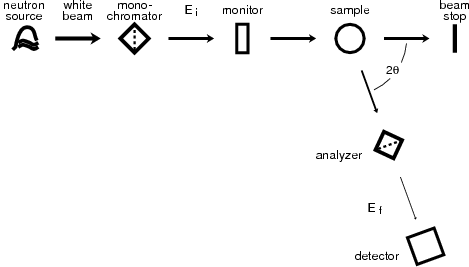
\includegraphics[width=0.7\textwidth]{img/Inelastic-neutron-scattering-basics.png}
\caption{Diagram of the basic principle of an inelastic neutron scattering experiment. $E_i$ is the incident energy, $E_f$ is the final energy.}
\label{fig:indirect-inelastic-diagram}
\end{figure}

In a time-of-flight (TOF) experiment, values for the incident and final energy can be calculated from the parameters of the neutron flight path in an instrument as shown in figure xx and is given by the equation:

\begin{equation*}
E_f = \frac{1}{2}mv^2 = \frac{1}{2}m ( L_2 / t_2 ) ^2 
\end{equation*}

Using the above formula it is easy to see that the energy transfer equation can be rewritten in terms of the instrument parameters as:

\begin{equation*}
\hbar\omega = E_i - E_f = \frac{1}{2}m_n[(L_1 / t_1-t_2)^2 - (L_1/t_2)^2]
\end{equation*}

%\section{Indirect Inelastic Data Analysis with Mantid}
%\subsection{Convert To Energy}
%\subsubsection{Energy Transfer}
%\subsubsection{Calibration}
%\subsubsection{Diagnostics}
%\subsubsection{Transmission}
%\subsubsection{$S(Q,\omega)$}
%\subsubsection{Moments}
%
%\subsection{Indirect Data Analysis}
%\subsubsection{ElWin}
%\subsubsection{MSD Fit}
%\subsubsection{Fury}
%\subsubsection{FuryFit}
%\subsubsection{ConvFit}
%\subsubsection{Calculate Corrections}
%\subsubsection{Apply Corrections}
%
%\subsection{Indirect Bayes}
%\subsubsection{ResNorm}
%\subsubsection{Quasi}
%\subsubsection{Stretch}
%\subsubsection{JumpFit}
%
%\subsection{Indirect Diffraction}
%
%\subsection{Indirect Simulation}
%\subsection{Indirect Load ASCII}
%
%\section{Structure and Hierarchy}
%
%%\section{Planning for the future}
%%\subsection{Conversion of routines into workflow algorithms}
%%\subsection{Better automated test coverage}
%%\subsection{Improved GUI structure and design}
%%\subsection{GUI support for VESUVIO}
%%\subsection{nMOLDYN integration into Mantid}
%%\subsection{Conversion of remaining Fortran routines}
%%\subsection{Better support for other facilities}
%%\subsection{Multiple scattering support}

\bibliographystyle{plain}
\bibliography{refs}
\end{document}